%%%%%%%%%%%%%%%%%%%%%%%%%%%%%%%%%%%%%%%%%%%%%%
%Lab report writeup based on template by Derek Hildreth
%%%%%%%%%%%%%%%%%%%%%%%%%%%%%%%%%%%%%%%%%%%%%%

%\documentclass[aps,letterpape,10pt]{revtex4}
\documentclass[aps,letterpaper,10pt]{article}
%\documentclass{article}

\usepackage{graphicx} % For images
\usepackage{float}    % For tables and other floats
\usepackage{verbatim} % For comments and other
\usepackage{amsmath}  % For math
\usepackage{amssymb}  % For more math
\usepackage{fullpage} % Set margins and place page numbers at bottom center
\usepackage{subfig}   % For subfigures
\usepackage[usenames,dvipsnames]{color} % For colors and names
\usepackage{fancyhdr} %headers
\usepackage{listings} %for code
\usepackage{color} %to color code
\usepackage{wrapfig} % for inline images

%Color and code setup
\definecolor{dkgreen}{rgb}{0,0.6,0}
\definecolor{gray}{rgb}{0.5,0.5,0.5}
\definecolor{mauve}{rgb}{0.58,0,0.82}
\definecolor{codebg}{rgb}{.95,.95,.98}

\lstset{ %
	language=Python, 
	tabsize=4, 
	numbers=left,
	numberstyle=\footnotesize,
	backgroundcolor=\color{codebg},
	breaklines=true,
	breakatwhitespace=true,
	basicstyle=\small,
	numberstyle=\tiny\color{black},
	showstringspaces=false,
	keywordstyle=\color{blue}, 
	stringstyle=\color{dkgreen},
	commentstyle=\color{gray},
	frame=single,
	title = \texttt{\lstname}
	}

%%%%%%%%%%%%

%HEADER FORMATING%%%%%%%%%%%%%
\pagestyle{fancy}
\headheight 10pt
\setlength{\headsep}{20pt}
\lhead{MPHY 396 - Prof. Armato\\ Homework 3}
\rhead{A. Athanassiadis\\Due 2/1/2012}
%%%%%%%%%%%%%%%%%%%%%%%%

%Custom Definitions%%%%%%%%%%%%%%%
\newcommand{\ttt}{\texttt}
%%%%%%%%%%%%%%%%%%%%%%%%

\begin{document}
\section{Problem 1}
\begin{figure}[!h]
\centering
\subfloat[Original Region]{\label{fig:3-1a}
\includegraphics[width=.30\textwidth]{3-1a.png}}\hspace{40px}
\subfloat[4-Connected Edge Tracking]{\label{fig:3-1b}
\includegraphics[width=.30\textwidth]{3-1b.png}}\\
\subfloat[8-Connected Edge Reduction]{\label{fig:3-1c}
\includegraphics[width=.30\textwidth]{3-1c.png}} \hspace{40px}
\subfloat[Edge Differences]{\label{fig:3-1d}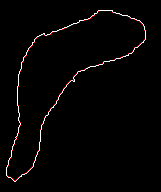
\includegraphics[width=.30\textwidth]{3-1d.png}}
\caption{Edge Tracking}
\label{fig:3-1}
\end{figure}
\vspace{-10px}
Figure \ref{fig:3-1a} shows the initial region under consideration.  Using the 4-connected edge tracking algorithm proposed in class, the edge in Figure \ref{fig:3-1b} was created: once the first `on' pixel (rastering across then down from the upper left) was identified, the region was tracked going counter-clockwise.  The edge was reduced using the \ttt{reduce\_edge()} function, which looked for redundant pixels in an 8-connected sense.  When implementing this, it is important to realize that some sets of points are necessary to retain even if they can be substituted by 8-connected points, because these `redundant' points are part of the region.  Therefore, I solved that all redundant steps were at right angles (odd difference) but only when the shorter edge would not exclude a part of the region.  This corresponds to cuts that are locally concave with respect to the region when going counterclockwise, or alternately when the difference between successive moves is positive.  The other key was to note that when two successive moves involved 3 and 0 (see \ttt{problem1.py} for direction maps), the 0 should be treated as a 4 in order to not cut through the region.  The result is shown in Figure \ref{fig:3-1c}.  Finally, the differences in the edges can be seen in Figure \ref{fig:3-1d}.  The overlap of both edges is given in white, and the pixels cut out from the 4-connected edge are shown in red.

Chain code for both edge chains are listed below in \ttt{problem1chain\#.txt} The perimeters of both regions were calculated based on the chain length, less two for the coordinates of the start pixel.  The results are given in \ttt{problem1.txt}.  As expected, the 8-connected edge is smaller than the 4-connected edge.
\lstinputlisting{problem1chain4.txt}
\lstinputlisting{problem1chain8.txt}
\lstinputlisting{problem1.txt}
\lstinputlisting{problem1.py}


\section{Problem 2}
\begin{figure}[!h]
\centering
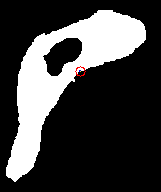
\includegraphics[width=.5\textwidth]{3-2a.png}
\caption{Bad Start Point}
\label{fig:3-2}
\end{figure}
The tracking algorithm used in Problem 1 will not successfully track a region's edge for arbitrary start points.  The next direction to search is always set as the direction one step counterclockwise from the move just made.  Therefore, the algorithm assumes that the first pixel was reached by rastering from upper left, and therefore that the first direction to check is one pixel up from the initial pixel.  Thus, if the start point is set somewhere on an underside of the image, the border tracking algorithm will be confused, as is evident in Figure \ref{fig:3-2}.  The start point for the tracking algorithm was the yellow point at the center of the red circle.  The four blue pixels around the yellow pixel are the border that it tracked, which just form a small $2\times2$ square including the start pixel.
\newpage
\lstinputlisting{problem2.py}

\section{Problem 3}
Depending on the task, there are various ways to fill a region based on the edge in Figure \ref{fig:3-1c} and preserve the hole in the original region.  One method is to completely fill the region and then perform an element-wise multiplication of the array containing the original figure, and that containing the filled region.  Because the two figures are binary, this will result in another binary image that only retains points common to the two regions.  This however seems less useful because it does not give the computer any new information that it did not have from the original figure. This could be used to determine the inner border though: the original region could be element-wise subtracted from the hole-less region.  This would produce an  image that consisted of the central hole being bright (1) and everything else appearing as background (0).  This image could then be used to track the inner edge of the region.  This method can be used recursively to track nested regions, and is generalizable when tracking regions in binary images.

Alternately, a second border tracking could be performed to find the border of the interior region.  The edge filling algorithm could then take this into account and keep track of `entrance' and `exit' pixels for a region, like the algorithm presented in class.  This smart filling would require a bit more computation time, but would give the computer more knowledge of the figure that it is analyzing.  Instead of separately tracking the interior boundary, another algorithm could calculate gradients in the original image, and then use the gradient image as a boundary image to perform a similar smart filling algorithm.
\newpage
\section{Problem 4}
\begin{figure}[!h]
\centering
\subfloat[Original Image]{\label{fig:3-4a}
\includegraphics[width=.33\textwidth]{3-4a.png}}\hspace{40px}
\subfloat[Identified Regions]{\label{fig:3-4b}
\includegraphics[width=.33\textwidth]{3-4b.png}}
\caption{Region Identification}
\label{3-4}
\end{figure}
The original image to be segmented is shown in Figure \ref{fig:3-4a}.  Initially guessing, a region labeling algorithm scanning from the top left corner should need to allocate 11 regions before adjusting the image using the equivalence table.  This is due to the separation of the two edges in the letter \textsf{H}, as well as the bottom curl in the letters \textsf{C} and \textsf{G}.  My algorithm processed this image and came up with the 7 distinct regions colored in image \ref{fig:3-4b}.  The number of components was determined by the number of entries in the equivalence table that point to themselves.  The output, including the equivalence table, are given in \ttt{problem4.txt}.  As expected, 11 distinct regions were discovered before remapping regions based on the equivalence table.

Note that to run this algorithm, the original image was padded with one pixel on each side, in order to identify regions that potentially include boundary pixels.  The padding was removed when returning the labeled image.

\lstinputlisting{problem4.txt}
\lstinputlisting{problem4.py}

\section{Appendix: Common Code}
Common functions used for these problems are contained in \texttt{segmentation.py}.
\lstinputlisting{segmentation.py}

\end{document} 